

\begin{figure}[hp]
    \centering
    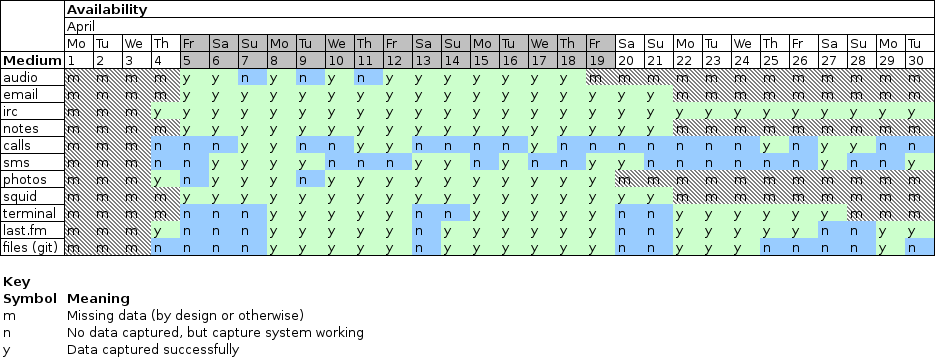
\includegraphics[width=1.0\textwidth]{personal/dataoverview}
    \caption{The availability of data from various sources}
    \label{fig:personal:dataoverview}
\end{figure}


These results describe data collected during the third iteration of sampling, which lasted roughly two weeks during April 2013.  Table~\ref{figure:personal:dataoverview}\td{make into a table} describes the availability of data per-day.

The period marked from Friday the 5th to Friday the 19th (inclusive) forms the sampling period described herein (with exceptions to this noted where made).  This was the period for which the on-line notebook was maintained along with other intrusive data collection techniques, though notably some methods continued due to their ease-of-use.

Audio data is missing for the 19th as sampling was initially intended to end the day before, however, for producing estimated word counts this was not used as other recording methods cover the data sources.  Though attempts were made to use the audio data, difficulties in automated processing meant that transcription (or precise word counts) were only possible using manual review (something only the subject could legally perform).  Word counts were instead based on an estimated words-per-minute.


This fifteen-day recording period covers 8,619 linguistic events, encompassing an estimated 980,000 words.  In total 3.4GB of data were collected, though the majority of this figure (2.3GB, 67\%) of this is audio data.  This is roughly in line with other life-logging studies \td{cite magazine article on mylifebits where they discuss storage sizes}.

The overall word count is changed massively by disabling the attention model, rising to roughly 5 million words.  As we shall see later, this is largely because the data sources and genres which dominate the data set are particularly heavily adjusted.  This raises the question of how we may ensure accuracy of attention models, something that shall be addressed in the discussion section below.




% ---------------------------------------------------------------------------
% \subsection{Variables}
Variables recorded on each linguistic event are based heavily on Lee's BNC index, augmented to take into account the attention index and word count estimates.  A summary of these is provided in Table~\ref{table:personal:variables}.  The `missing' column describes the proportion of rows missing this field, either because it is not applicable, or because insufficient data was recorded to complete it with confidence.

The variables `source2' and `duration' have missing values exclusively due to non-applicability.  As such they have been integrated into (complete) summary variables for analysis, forming the computed words and computer genre in an effort to unify measurement of spoken and written material, and increase the specificity of the data source recorded.

Though part of the initial purpose 


\begin{table}[hp]
\centering
    \begin{tabular}{ | l | c | p{7cm} |}
    \hline
    \textbf{Variable} & \textbf{Missing} & \textbf{Description} \\ \hline
   
    source              & - & The data source (email, audio, etc.) \\ \hline
    source2             & 34.3\% & Any origin data from within the source (i.e. the caller in a phone conversation, sender for email) \\ \hline
    day                 & - & Day of the month sampled \\ \hline
    mode                & - & Spoken or Written \\ \hline
    circulation status  & - & Exact circulation, or `h', `m', `l' following Lee's guidelines\\ \hline
    portion read        & - & The attention index mentioned above \\ \hline
    informal genre      & - & Free-coded genre \\ \hline
    medium              & - & The form of the language used.  Usually the same as the source. \\ \hline
    % ...
    title               & - & The title of the document, or an identifier for the text \\ \hline
    author              & 18.0\% & The author[s] of the text\\ \hline
    author age          & 97.2\% & The age of the author[s] \\ \hline
    author sex          & 97.1\% & The sex of the author[s] \\ \hline
    author type         & - & An indication of the type of entity authoring the text.  Follow's Lee's coding for \textbf{s}ingle, \textbf{m}ultiple, and \textbf{c}ommercial\\ \hline
    produced/consumed   & - & During the transaction, was text produced, consumed, or engaged in interactively \\ \hline 
    % \hline
    words               & 2.8\% & Authoritative word count\\ \hline
    duration            & 97.2\% & Authoritative duration for spoken data\\ \hline
    computed words      & - & Estimated word count, merging durations and word counts above\\ \hline
    computed genre      & - & A composite of the medium and the informal genre, intended as a more specific genre representation \\
    \hline
    \end{tabular}
\caption{A summary of variables sampled}
\label{table:personal:variables}
\end{table}





% ---------------------------------------------------------------------------
\subsection{Activities}
During the sampling period, all work surrounding the personal corpus case study was stopped, in favour of other, ongoing, projects.  Other than this intervention, work continued as normal, which for this period involved significant amounts of development on the LWAC downloader tool.

\til{How much to write about those two weeks?}
% TODO: more about general life in that period






% ---------------------------------------------------------------------------
\subsection{Distribution}
Quantitative data about time and other super-simple breakdowns here



\begin{figure}[hp]
    \centering
    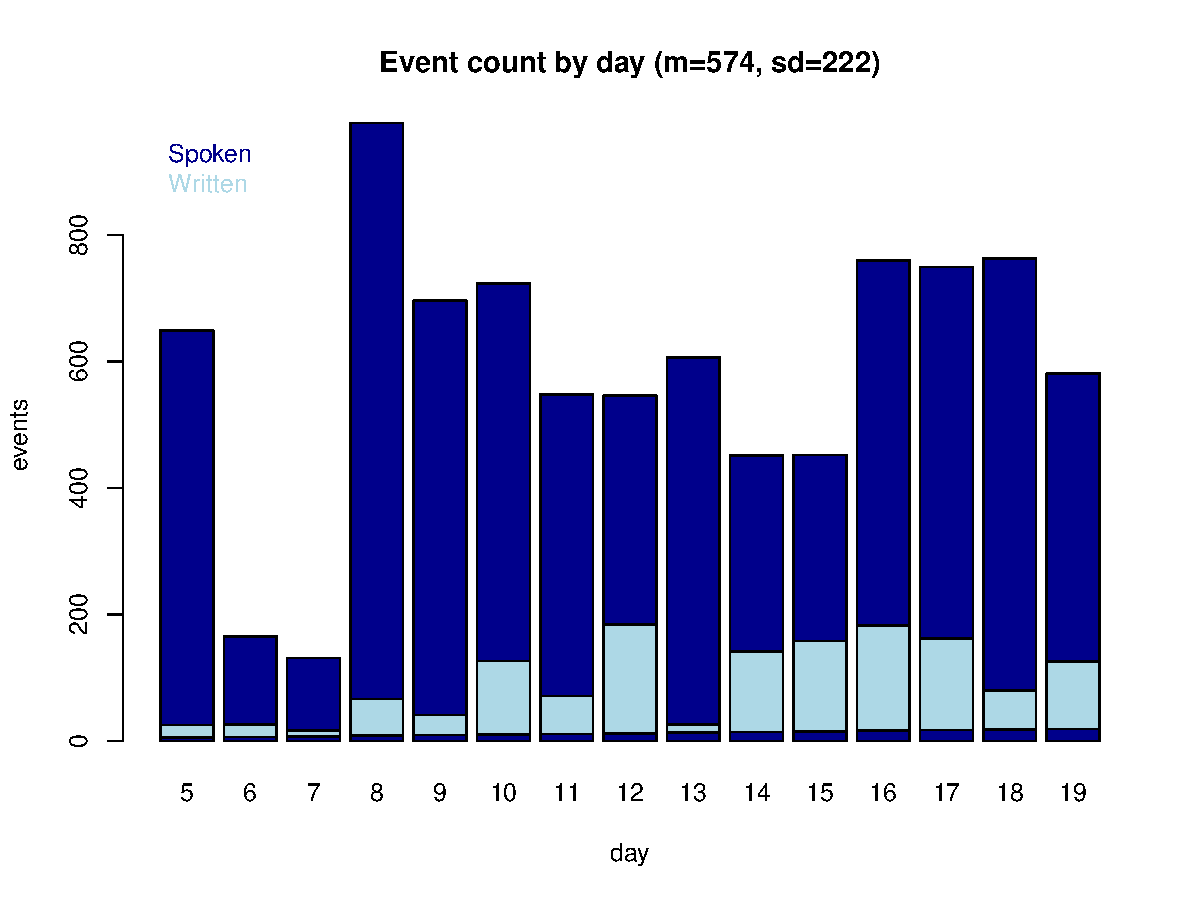
\includegraphics[width=0.8\textwidth]{personal/ebyday}
    \caption{Daily event frequencies}
    \label{fig:personal:eventcountbyday}
\end{figure}


Figure~\ref{fig:personal:eventcountbyday} shows the number of events recorded each day.  It shows event counts between 124 and 969, with much of the variation being expressed in terms of written data.  \td{a large amount of that 969 is terminal stuff from developing lwac all day}.

Contrary to expectations, and in part due to large aomunts of terminal and web use during software development work, the majority of daily language use is written.  This is contrasted by Figure~\ref{fig:personal:wordcountbyday}, which indicates that spoken events are likely to expunge greater amounts of words in a single event (spoken median is 128 words, vs. 27 words for written).  This is largely explainable by a penchant for consuming broadcast media (especially spoken radio), which have large amounts of ongoing spoken content.

% > mean(dat[which(dat$mode == 's'),]$computed_words)
% [1] 307.464
% > mean(dat[which(dat$mode == 'w'),]$computed_words)
% [1] 76.68702
% > sd(dat[which(dat$mode == 's'),]$computed_words)
% [1] 938.2
% > sd(dat[which(dat$mode == 'w'),]$computed_words)
% [1] 196.6995
% 


\begin{figure}[hp]
\centering
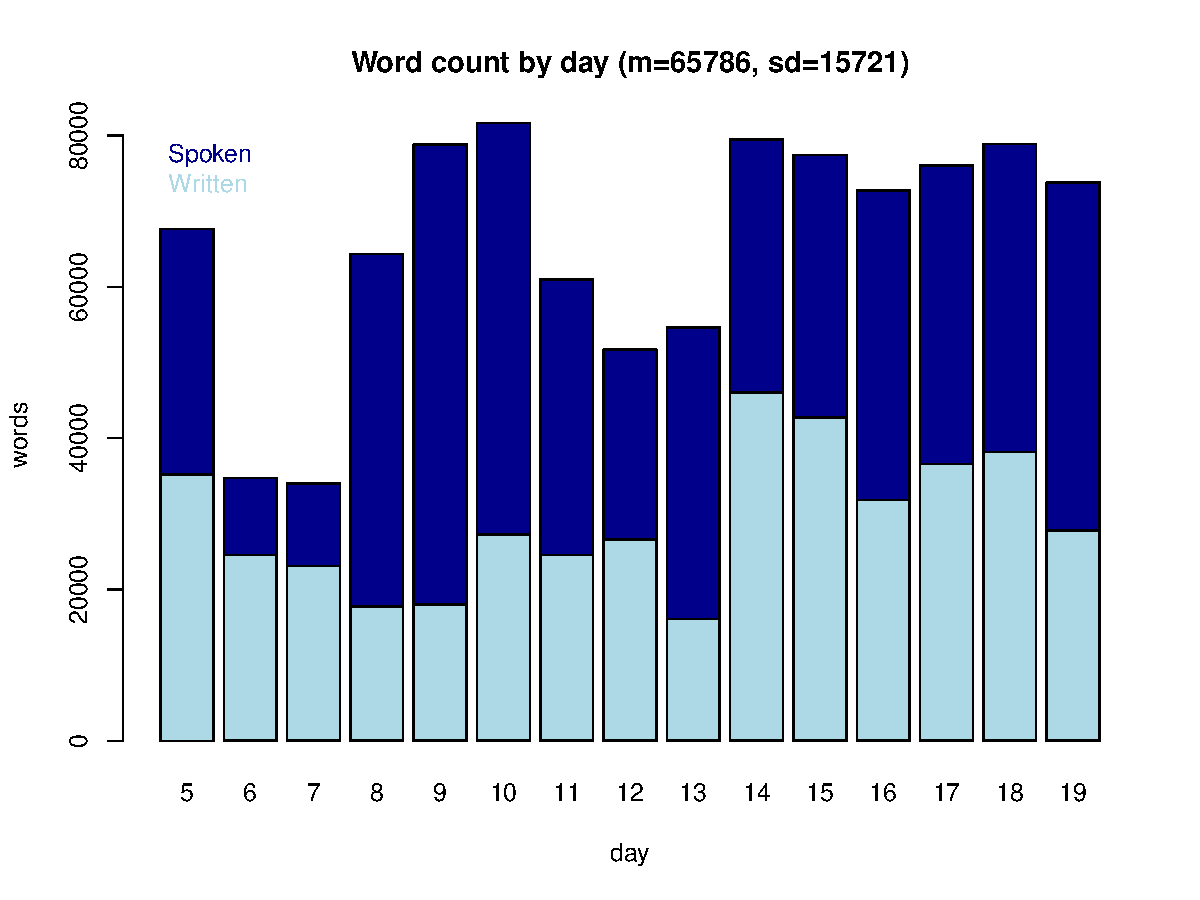
\includegraphics[width=0.8\textwidth]{personal/cbyday}
\caption{Daily word counts}
\label{fig:personal:wordcountbyday}
\end{figure}

As shown in Figure~\ref{fig:personal:eventcountbyday}, the event count as broken down by day shows that between 35,000 and 80,000 words were used each day.  As we shall see later, this is mainly explainable by way of broadcast media and web page views.  It is notable that weekends fall upon days 6,7,13 and 14.  There is no significant pattern by day.

Before this study it was conjectured that the vast majority of all language used would be 



\til{More fun breakdowns.  Take some plots from presentation. plot and comment on the distribution of some larger features throughout the data}





% ---------------------------------------------------------------------------
\subsection{Events}

\til{Plot event by source, bar plot}
\begin{figure}[hp]
    \centering
    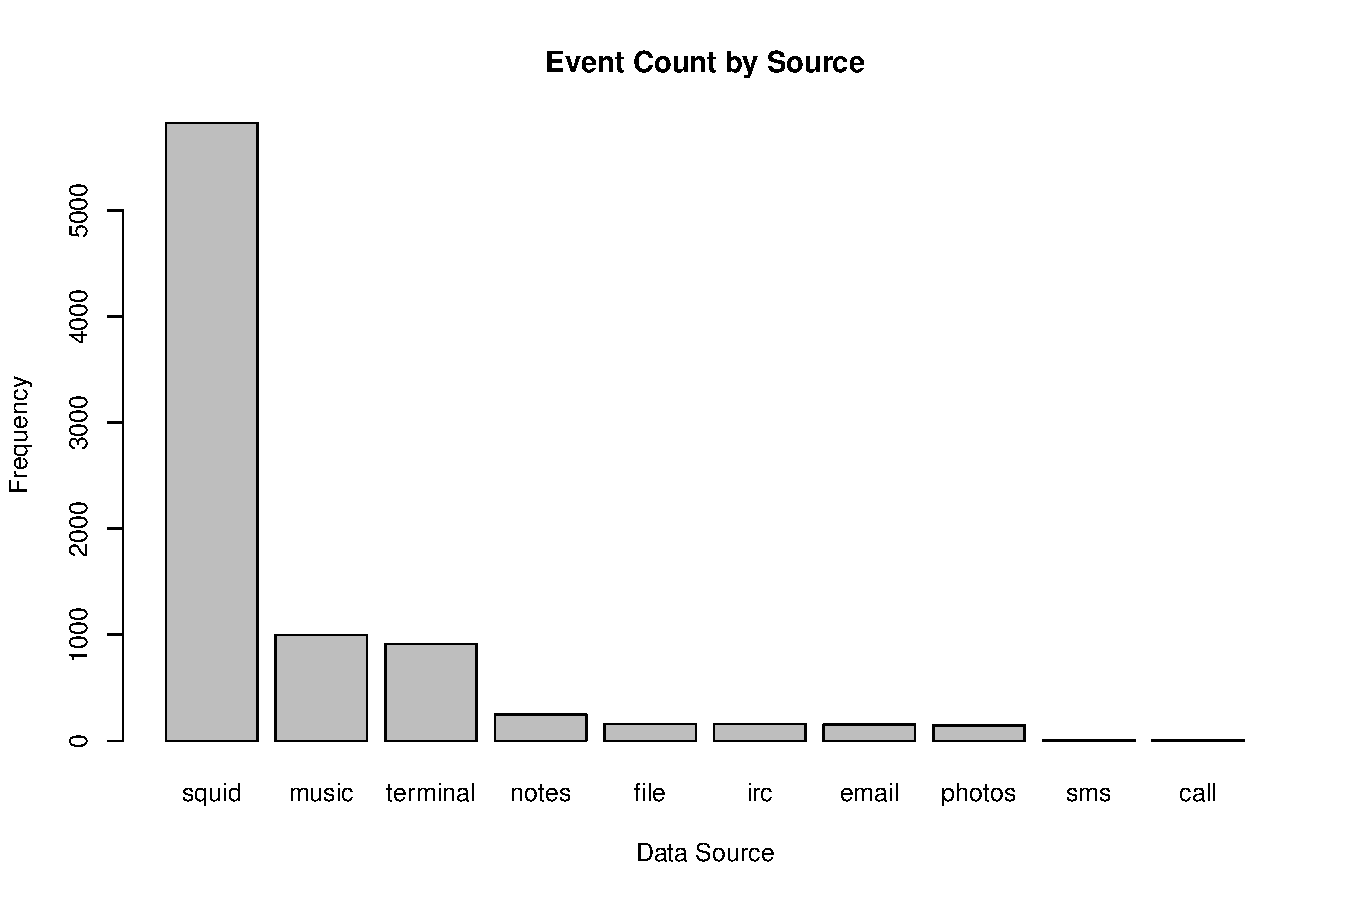
\includegraphics[width=0.8\textwidth]{personal/ebysource}
   %  \begin{verbatim}
   %  call    email     file      irc    music    notes   photos      sms 
   %    14      184      279      266     1433      272      152       28 
   % squid terminal 
   %  6076     1214 
   %  \end{verbatim}
    \caption{Event count by source}
    \label{fig:personal:eventsbysource}
\end{figure}

The proportions described in Figure~\ref{fig:personal:eventsbysource}\td{make into bar graph} are likely a very individual trait of the subject.  They exhibit a number of properties that would be significantly affected not only by daily routine, but also the specific work being completed at the time of the sample (the implications of this on scientific validity are discussed below in section~\ref{}\td{ref}).

Particularly curious is the large number of terminal, web (squid), and music events.  These are partially explainable by the work being completed at the time of the study, as the subject was developing software, listening to music whilst doing so and using many web references as documentation.  The subject also uses a GUI on his computer that mandates use of terminals for many tasks (this is doubtless atypical).



\begin{table}[ht]
\centering
\begin{tabular}{rr}
      \hline
      Computed Genre & Events \\ 
      \hline
      web/entertainment/social & 2598 \\ 
      web/music & 708 \\ 
      display/output & 627 \\ 
      music/punk & 587 \\ 
      web/reference & 421 \\ 
      web/shopping & 388 \\ 
      display/interactive & 285 \\ 
      web/academic & 280 \\ 
      web/tech & 218 \\ 
      web/outdoors & 180 \\ 
      web/video streaming & 167 \\ 
      irc/informal/discussion & 159 \\ 
      music/guitar & 147 \\ 
      web/academic/reference & 142 \\ 
      web/tech/reference & 116 \\ 
      web/news & 105 \\ 
      file/ruby code &  82 \\ 
      music/metal &  73 \\ 
      music/pop &  68 \\ 
      music/rock &  67 \\ 
      web/hosting &  54 \\ 
      file/documentation &  49 \\ 
      web/comedy &  49 \\ 
      web/social &  49 \\ 
      web/product support &  48 \\ 
      product/packaging &  43 \\ 
      web/tech/academic &  40 \\ 
      TV/comedy &  39 \\ 
      web/outdoors/reference &  36 \\ 
      email/academic &  34 \\ 
      email/advertising &  28 \\ 
      web/entertainment &  28 \\ 
      email/personal &  26 \\ 
      file/config &  24 \\ 
      email/business &  22 \\ 
      speech/discussion &  22 \\ 
      speech/informal &  21 \\ 
      web/comedy/social &  21 \\ 
      email/orders &  20 \\ 
      speech/service &  19 \\ 
      web/search &  19 \\ 
      email/spam &  17 \\ 
      music/blues &  17 \\ 
      speech/greeting &  16 \\ 
      web/fitness &  16 \\ 
      web/tech/news &  15 \\ 
      TV/Entertainment &  14 \\ 
      speech/info &  14 \\ 
      web/tech/shopping &  14 \\ 
      web/reference/academic &  13 \\ 
      TV/news &  12 \\ 
      radio/music &  12 \\ 
      radio/news &  12 \\ 
      sign/info &  11 \\ 
      web/art &  11 \\ 
      web/music/shopping &  11 \\ 
      music/folk/metal &   9 \\ 
      music/progressive &   9 \\ 
      TV/entertainment &   8 \\ 
      email/technical &   8 \\ 
      sign/info/instruction &   8 \\ 
      speech/ephemera &   8 \\ 
      web/banking &   8 \\ 
      music/country/rock &   7 \\ 
      music/fusion &   7 \\ 
      sign/product info &   7 \\ 
      book/info &   6 \\ 
      sign/advertising &   6 \\ 
      TV/documentary &   5 \\ 
      flyer/advertising &   5 \\ 
      notes/note &   5 \\ 
      product/info &   5 \\ 
      speech/parting &   5 \\ 
      web/advertising &   5 \\ 
      web/conspiracy &   5 \\ 
      box/address &   4 \\ 
      flyer/info/advertising &   4 \\ 
      radio/news/entertainment &   4 \\ 
      sms/informal &   4 \\ 
      web/blogs &   4 \\ 
      web/games &   4 \\ 
      web/news/social &   4 \\ 
      web/reference/social &   4 \\ 
      web/reference/travel &   4 \\ 
      web/reference/woodwork &   4 \\ 
      web/shopping/investment &   4 \\ 
      web/tech/utility &   4 \\ 
      web/utility &   4 \\ 
      TV/advertising &   3 \\ 
      application/info &   3 \\ 
      file/js code &   3 \\ 
      flyer/menu &   3 \\ 
      music/country &   3 \\ 
      phone/ &   3 \\ 
      sign/advertising/info &   3 \\ 
      sms/info &   3 \\ 
      speech/organisation &   3 \\ 
      speech/request &   3 \\ 
      web/health &   3 \\ 
      web/news/tech &   3 \\ 
      application/info/status &   2 \\ 
      book/packaging/book title &   2 \\ 
      map/info &   2 \\ 
      music/indie &   2 \\ 
      paper slip/invoice &   2 \\ 
      phone/informal &   2 \\ 
      poster/advertising &   2 \\ 
      radio/News &   2 \\ 
      speech/Discussion &   2 \\ 
      speech/informal/discussion &   2 \\ 
      web/comedy/entertainment &   2 \\ 
      web/entertainment/images &   2 \\ 
      web/entertainment/news &   2 \\ 
      web/entertainment/puzzles &   2 \\ 
      web/game &   2 \\ 
      web/tech/social &   2 \\ 
      TV/advertising/info &   1 \\ 
      TV/documentary/entertainment &   1 \\ 
      TV/info &   1 \\ 
      TV/music &   1 \\ 
      TV/sport &   1 \\ 
      application/album listing &   1 \\ 
      application/buttons/info &   1 \\ 
      application/update &   1 \\ 
      book/ &   1 \\ 
      book/packaging/book blurb &   1 \\ 
      box/packaging &   1 \\ 
      card/info &   1 \\ 
      cheque/info &   1 \\ 
      clothing/packaging &   1 \\ 
      display/info &   1 \\ 
      display/info/status &   1 \\ 
      file/html code &   1 \\ 
      film/Entertainment &   1 \\ 
      game/discussion &   1 \\ 
      game/game &   1 \\ 
      music/classical &   1 \\ 
      music/electronica &   1 \\ 
      music/music &   1 \\ 
      music/pop/metal &   1 \\ 
      notes/agenda/minutes &   1 \\ 
      notes/diagram &   1 \\ 
      noticeboard/advert &   1 \\ 
      paper slip/info &   1 \\ 
      phone/info &   1 \\ 
      poster/info &   1 \\ 
      poster/menu &   1 \\ 
      product/instruction/info/packaging &   1 \\ 
      radio/News/entertainment &   1 \\ 
      sign/ &   1 \\ 
      sign/instruction &   1 \\ 
      sign/map &   1 \\ 
      sign/menu &   1 \\ 
      sms/ &   1 \\ 
      speech/Informal &   1 \\ 
      speech/Inquiry &   1 \\ 
      speech/discussion/academic &   1 \\ 
      speech/info/discussion &   1 \\ 
      speech/question &   1 \\ 
      speech/service/discussion &   1 \\ 
      taxdisc/info &   1 \\ 
      vehicle/branding/sign &   1 \\ 
      vehicle/info/advertising &   1 \\ 
      video/info/academic &   1 \\ 
      video/info/advertising &   1 \\ 
      web/downloads &   1 \\ 
      web/games/news &   1 \\ 
      web/info/advert &   1 \\ 
      web/reference/entertainment &   1 \\ 
      web/reference/military &   1 \\ 
      web/reference/outdoors &   1 \\ 
      web/reference/shopping &   1 \\ 
      web/tech/hosting &   1 \\ 
       \hline
\end{tabular}
\caption{Event frequency by computed genre}
\label{table:personal:eventcountbygenre}
\end{table}


Table~\ref{table:personal:eventcountbygenre} shows a breakdown of event frequencies by computed genre \td{probably exclude hapaxes to shorten the table?} (which includes the source).  This shows a somewhat predictable zipfian distribution of genres surrounding a number of themes:

\begin{itemize}
    \item Daily events, such as reading social media websites
    \item Short events, such as consuming single programs of media (especially songs due to additive effects with the above)
    \item Any of the above that are particularly surrounding personal interests of the subject
\end{itemize}

Clearly, the last of these is the most obvious and desirable effect of building a corpus using this method.  The overwhelming prevalence of \texttt{web/entertainment/social} events may be explained (rather embarrassingly) by one website, which displays a single image per page (along with socially-contributed captions), and thus demands a lot of page reloads for relatively little content.








% ---------------------------------------------------------------------------
\subsection{Word Counts}

\begin{table}[ht]
    \centering
    \begin{tabular}{rrrrrrrr}
        \hline
        & 5\% & 10\% & 20\% & 50\% & 70\% & 90\% & 95\% \\ 
        \hline
        1 & 0.00 & 0.00 & 8.90 & 27.85 & 74.00 & 217.00 & 354.88 \\ 
        \hline
    \end{tabular}
    \caption{Percentiles for words-per-event.}
    \label{table:personal:wordsperevent}
\end{table}

Word counts were established either directly, or by assuming an 80 word-per-minute speech ratetd{cite where this figure was pulled from, mention that song lyric estimates also back it up}.  Table~\ref{table:personal:wordsperevent} shows that the distribution of word count per event is heavily skewed towards the lower end, with the median being 27 words per event.

This figure also reflects the degree to which the attention model affects results---disabling calculations for this, the distribution of word counts is affected significantly by the largest source of data, web pages, becoming 442 words.  Most pages are, even compared to other types of event in the corpus, read only partially (often graphical clues indicate which portions to read, especially since most people revisit websites more than they visit new ones).









% ---------------------------------------------------------------------------
\subsection{Comparisons}
\til{Table of high-level genres for the two (align them).

This could be done by re-coding existing genres or by fitting both to higher-level ones (the latter might be clearer and less work)}



% Comparisons against BNC for genres, word counts etc.  Also extract demographic info from BNC for more targeted comparison
At a large scale, there are some obvious differences between the personal corpus and the BNC's selection.

One of the most striking of these is the rate of broadcast media consumption, which forms a full 50\% of the subject's spoken word count, yet only 10\% of the BNC's.  There is a fair argument to say that many people of a similar age, who grew up surrounded by online streaming services and easy access to cheap receiving devices, will share this disparity.

A less compelling difference is exhibited between the rate of spoken conversations---our subject's spoken data was 20\% conversational, whereas the BNC contains 40\% conversational data (as a proportion of its spoken component).  The degree to which this applies to others is difficult to estimate, since (contrary to the verbiage of this thesis) the subject may simply be unusually laconic.



Arguments for the diversity of texts within corpora are driven only vaguely by the quantitative findings of this study due to its restricted inter-person relevance.  Nonetheless, some trends were identified which could reasonably be expected to extend to many others in a similar culture.

Inspecting the selection of genres yields a diversity not covered in many corpora.  Though notably the BNC is quite good at this, covering many brochures and other such texts\td{examples}, it hardly represents the amount of times thanks were exchanged for holding a door open, bottles, cans and other labels were read (particularly addresses on mail), or a tax disc was checked.  It would seem that a corpus purporting to cover a large population would be awash with weirder texts, especially as those less academic than the subject here are likely to have relatively higher proportions of them in their corpora.

A particularly compelling argument is made for the inclusion of song lyrics.  These are a large portion of the corpus collected here \td{how big}, and often spawn sayings, memes and linguistic affectations that can last decades in popular culture (\textit{will you do the Fandango?}).  It's also notable that this is one of the easier things to sample and music use by the population is meticulously documented and studied by the industry already (often in publicly available lists).  In the case of music, use of English as a lingua franca would see its influence spread far beyond the bounds of a national corpus (as well as absorbing influences from other national flavours of the language% Gasolina or Shakira's spanish singing?
).









% ---------------------------------------------------------------------------
\subsubsection{Genres Absent from the Corpus}
There are a number of genres absent from the corpus that are listed in the BNC.  Examples of this that are unlikely to change if the sampling period is extended indicate lifestyle differences and, in sum, indicate the likely representativeness of the BNC relative to the subject.  Where a genre is seen as likely to be represented given sufficient time, they are evidence that the sampling period was insufficient (something that the BNC's breadth mitigates).

Comparisons were performed between the list of composite source/genres given in Table~\ref{table:personal:wordsperevent} and Lee's genre listings.  Where any overlap was seen, a genre was discounted entirely.


\begin{table}[ht]
    \centering

    \begin{tabular}{ |l|l| }
        \hline
        Medium & Genre Category \\ \hline
        \multirow{5}{*}{Spoken (\texttt{S\_})} 
                                & classroom \\
                                & courtroom \\
                                & demonstratn \\
                                & interview* \\
                                & lect* \\
                                & sermon \\
        \hline
        \multirow{5}{*}{Written (\texttt{W\_})} 
                                & humanities\_arts \\
                                & ac* (all but tech\_engin) \\
                                & biography \\
                                & essay* \\
                                & fict\_poetry \\
                                & hansard \\
                                & newsp\_*\_sport \\
                                & pop\_lore \\
                                & religion \\
        \hline
    \end{tabular}
    \caption{Major categories missing from the personal corpus but present in the BNC.}
    \label{table:personal:missingcatspersonal}
\end{table}


The 11 (of 24) top-level categories missing entirely are summarised in Table~\ref{table:personal:missingcatspersonal}.  Of those spoken, only interviews and lectures are likely to ever be encountered during a longer sampling period.  The former of these would require a sampling period of years for most subjects.

Written material is more comprehensively covered, with 15 of 46 genres missing.  Worth noting is that, whilst newspaper articles are absent from the corpus in their original form, many of the same genre were read online (with the exception of sports articles).  




\til{Compare large-scale genres}

% ---
As expected, the genres identified within the personal corpus are an imperfect subset of those featured in the BNC.  Following Lee's index, there are no magazines, religious texts, newspapers, dramatic scripts, school or university essays, texts on the subject of commerce/economics or academic texts in many fields.  Newspapers alone comprise 9.9\% of the BNC, implying that caution should be exercised before applying any findings from the BNC to any single subject. % However, another criticism could be that the BNC is 100 times the size...

It is unfortunate that the BNC, even with Lee's annotation, lacks sufficient detail to create a demographic subset focused around the status of the subject covered here.

%---

Particularly interesting are instances where the hierarchical categorisation of the BNC indicates that both corpora have sampled from the same sources, yet the resulting within-category proportions differ.  

\til{recode data along lee's lines and pick these out}






